\section{Game structure}

\subsection{Game modes}
\noindent Project-Scopes offers two main game modes:
\begin{itemize}
	\item[-] \textbf{local mode} - in this mode, players are playing on single machine and using the same controller. Each player is involved in the game in real time and watching the game with exactly the same perspective as others (the image is not splitted).
	\item[-] \textbf{LAN mode} - in this mode player has the ability to connect to the game via the LAN network from a different, separate machine with its own controller and display. Players connected in this way are still participating in the game simultaneously in real time. Image generated for the players is the same, and it is broadcasted on their local displays.
\end{itemize}

\subsection{Interface}

\subsubsection{Menu}
\noindent Main menu appears after game starts. It offers the possibility to choose the game mode and, depending on the mode selected, the ability to set the configuration parameters of the players and the game itself.

\subsubsection{Screens}
\noindent The main screens, making up the game, are:
\begin{itemize}
	\item[-] \textbf{menu screen} - allows to choose a game mode
	\item[-] \textbf{configuration screen} - allows to set available gameplay parameters in selected mode
	\item[-] \textbf{wait for players screen} - in LAN mode means that player is ready for a game and waits for other players
	\item[-] \textbf{gameplay screen} - shows the actual gameplay
	\item[-] \textbf{pause screen} - can be launched from gameplay screen, means that the game is paused and waits for resume or close
	\item[-] \textbf{next round screen} - shows the winner of the round
	\item[-] \textbf{game over screen} - shows a table of players and points for each player position after last round end
\end{itemize}
\subsubsection{Controls}
\noindent One player needs two controller buttons to play.

\newpage
\subsection{Flowboard}
\begin{center}
	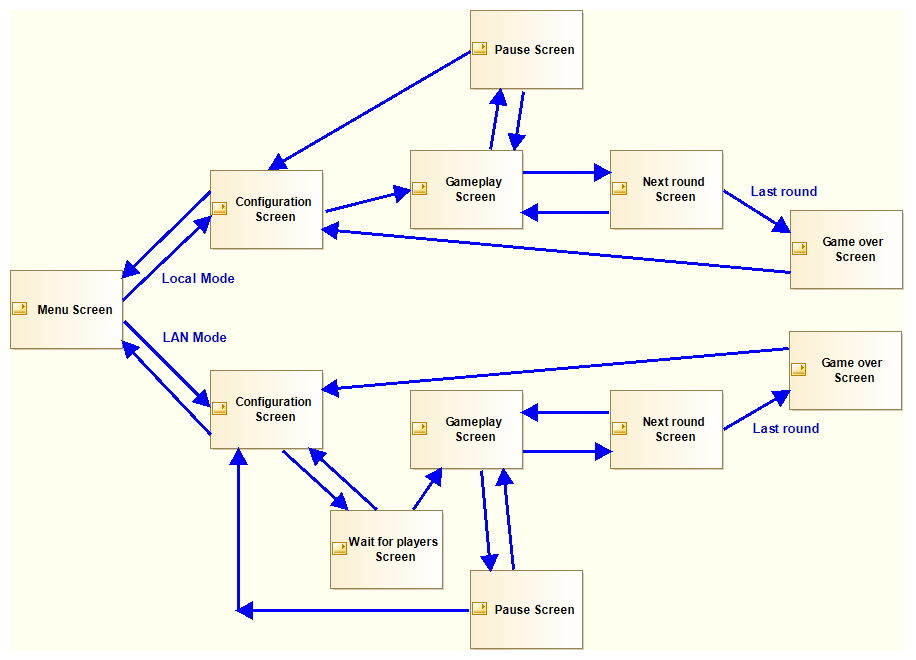
\includegraphics[width=\textwidth]{flowboard}
\end{center}